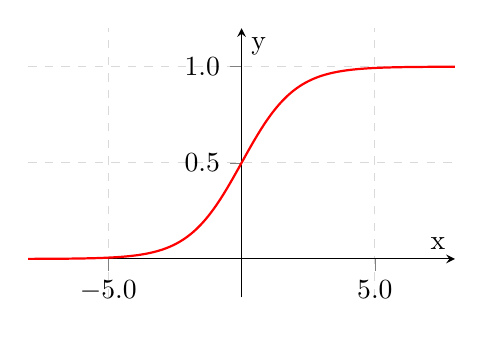
\begin{tikzpicture}
  \begin{axis}[
      legend pos=north west,
      axis x line=middle,
      axis y line=middle,
      x tick label style={/pgf/number format/fixed,
        /pgf/number format/fixed zerofill,
        /pgf/number format/precision=1},
      y tick label style={/pgf/number format/fixed,
        /pgf/number format/fixed zerofill,
        /pgf/number format/precision=1},
      grid = major,
      width=7cm,
      height=5cm,
      grid style={dashed, gray!30},
      xmin=-8,     % start the diagram at this x-coordinate
      xmax= 8,    % end   the diagram at this x-coordinate
      ymin= -0.2,     % start the diagram at this y-coordinate
      ymax= 1.2,   % end   the diagram at this y-coordinate
      %axis background/.style={fill=white},
      xlabel=x,
      ylabel=y,
      tick align=outside,
      enlargelimits=false]
    % plot the stirling-formulae
    \addplot[domain=-8:8, red, thick,samples=500] {1/(1+exp(-x))};
  \end{axis}
\end{tikzpicture}
